\documentclass{standalone}
\usepackage{tikz}
\begin{document}

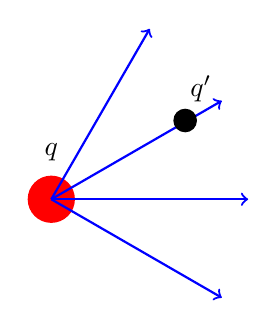
\begin{tikzpicture}
    % Partícula fuente
    \fill[red] (0,0) circle (0.3cm);
    \node at (0,0.6) {$q$};

    % Líneas de campo eléctrico
    \foreach \angle in {-30,0,30,60} {
        \draw[->, thick, blue] (0,0) -- (\angle:2.5);
    }

    % Partícula afectada
    \fill[black] (1.7,1.) circle (0.15cm);
    \node at (1.9,1.4) {$q^\prime$};

\end{tikzpicture}

\end{document}
